\subsection{Q15} \label{sec:q15}

For our filter design, fixed format number format called Q is used. Unlike floating point numbers, Q-format numbers require only standard integer ALU to perform rational number calculations. This means that we do not need to add an FPU to our design which requires additional power.

Q format numbers are represented using the Q notation which is written as Q$m,n$ where $m$ is the number of bits set aside to designate the two's complement integer portion of the number, and $n$ is the number of bits used to designate the fractional portion of the number.

In our case, we use simplified notation Q$n$ since we assume that the numbers are normalized into the range of $[-1, 1)$. Notice that this assumption does not affect the generality of the filter, but it simplifies the multiplication operation because the multiplication result never exceeds the range of $[-1, 1)$.

\begin{figure}[ht]
	\centering
	
\includegraphics[scale=1.5]{images/q7}
	\caption{Comparison between integer and Q7 format.}
	\label{fig:q7}
\end{figure}

Figure \ref{fig:q7} shows the comparison between two's complement integer and Q7 numbers. The only difference between the two is the weight assigned for each bit.

\subsection{Filter Characteristics}

\begin{figure}[ht]
	\centering
	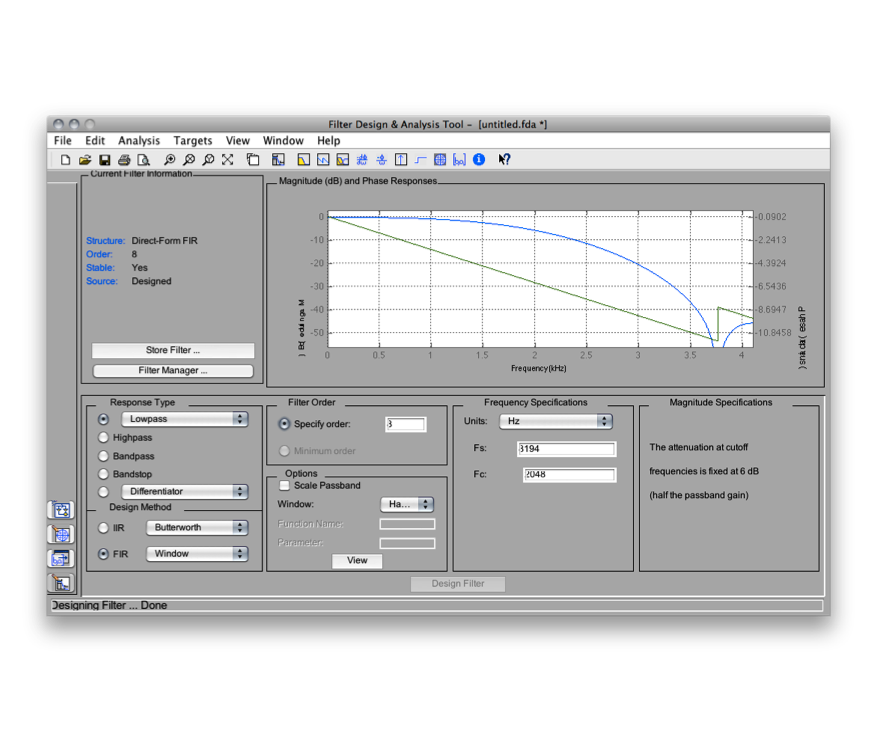
\includegraphics[scale=1]{images/matlab}
	\caption{Matlab.}
	\label{fig:matlab}
\end{figure}
